\documentclass{beamer}
\usepackage{amsmath}
\usepackage{amssymb}
\usepackage{geometry}
\usepackage{graphicx}
\usepackage{url}
\usepackage{xcolor}

% some latex magic for correcting apostrophe issue in verbatim mode
\makeatletter
\let \@sverbatim \@verbatim
\def \@verbatim {\@sverbatim \verbatimplus}
{\catcode`'=13 \gdef \verbatimplus{\catcode`'=13 \chardef '=13 }} 
\makeatother

\begin{document}

%---------------------------------------------
\begin{frame}
\large
Lecture 3:\\
Descriptive Statistics\\
STAT 310, Spring 2021
\normalsize
\end{frame}

%---------------------------------------------
\begin{frame}{Measures of Central Tendency}
Let $x_1, x_2, \cdots, x_n$ be observations of a sample of size $n$.  The \textbf{sample mean} is given by 
\begin{align*}
\bar{x} = \frac{1}{n}\sum_{i=1}^n x_i = \frac{x_1 + x_2 + \cdots + x_n}{n}
\end{align*}

\vspace{15pt}
\textbf{Ex}: The heights of 5 individuals: 63, 64, 66, 72, 62. 
\begin{align*}
\bar{x} = \frac{63 + 64 + 66 + 72 + 62}{5} = 65.4
\end{align*}
\end{frame}

%---------------------------------------------
\begin{frame}{Measures of Central Tendency}
\vspace{-1cm}
The \textbf{sample median} of a set of observations is the middle value when values are ordered from smallest to largest.\\
\vspace{20pt}

\textbf{Ex}: ($n$ odd) Find the median of $63, 64, 66, 72, 62$.\\
%\vspace{2cm} 
\medskip
{\color{blue}
First, order the data: $62, 63, 64, 66, 72$\\
median $= 64$\\
}
\vspace{10pt}

\textbf{Ex}: ($n$ even) Find the median of $63, 64, 66, 72, 62, 77$.\\
\medskip
{\color{blue}
First, order the data: $62, 63, 64, 66, 72, 77$\\
median $= (64+66)/2 = 65$\\
}
\end{frame}

%---------------------------------------------
\begin{frame}[fragile]{Measures of Central Tendency}
%\vspace{-1cm}
The median is resistant to outliers, while the mean is affected by outliers.\\
\vspace{10pt}
\textbf{Ex}: How do the mean and median compare for the sample:\\ $62, 63, 64, 66, 72, 1000$?\\
\begin{verbatim}
> x <- c(62, 63, 64, 66, 72, 1000)
> mean(x)
[1] 221.1667
> median(x)
[1] 65
\end{verbatim}
{\color{blue}
The sample mean is much larger than the median, since it is affected by the outlier.  The median is a better measure of central tendency in this example.
}
\end{frame}

%---------------------------------------------
\begin{frame}{Measures of Central Tendency}
%\vspace{-3cm}
Compare the mean and median for distributions that are symmetric, skewed right, and skewed left.\\
\vspace{20pt}
\centering
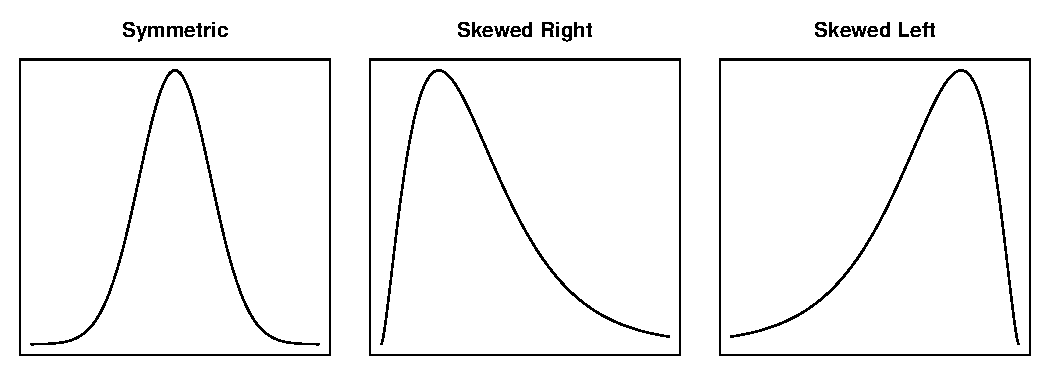
\includegraphics[scale=0.6]{figure/distributions.pdf}
\end{frame}

%---------------------------------------------
\begin{frame}{Quartiles}

\begin{itemize}
\item The \textbf{first quartile}, denoted by $Q_1$, is the value such that 25\% of the data falls below, i.e., the $25^{th}$ percentile.
\item The \textbf{third quartile}, denoted by $Q_3$, is the value such that 75\% of the data falls below, i.e., the $75^{th}$ percentile.
\item Note that the second quartile, $Q_2$, is the median.
\end{itemize}
\vspace{10pt}

A method for finding $Q_1$ and $Q_3$ by hand:
\begin{enumerate}
\item Order the data from smallest to largest
\item Divide the data into two sets using the median
\item $Q_1$ is the median of the first half, and $Q_3$ is the median of the second half\\
\end{enumerate} 
\end{frame}

%---------------------------------------------
\begin{frame}{Quartiles}
\vspace{-3cm}
\textbf{Ex}: Find $Q_1$ and $Q_3$ for the following sample of $n=10$ heights of individuals:\\ $68, 76, 66, 63, 70, 66, 71, 71, 64, 71$\\
% \medskip
% {\color{blue}
% \emph{Solution:}\\
% First, order the data: $63, 64, 66, 66, 68, 70, 71, 71, 71, 76$\\ 
% \bigskip
% median $= (68+70)/2 = 69$\\
% $Q_1 = 66$\\
% $Q_3 = 71$\\
% }
\end{frame}

\begin{frame}[fragile]
Useful R commands:
\small
\begin{verbatim}
> x <- c(68, 76, 66, 63, 70, 66, 71, 71, 64, 71)
> summary(x) 
   Min. 1st Qu.  Median    Mean 3rd Qu.    Max. 
   63.0    66.0    69.0    68.6    71.0    76.0 
> mean(x)
[1] 68.6
> median(x)
[1] 69
> min(x)
[1] 63
> max(x)
[1] 76
> sort(x)
 [1] 63 64 66 66 68 70 71 71 71 76
\end{verbatim}
\end{frame}

%---------------------------------------------
% \begin{frame}[fragile]{Percentiles}
% The more general $100 \cdot p^{th}$ \textbf{percentile}, where $0 \leq p\leq 1$, is the value such that $100 \cdot p$\% of the data falls below.  A related term is \textbf{quantile}; for example, the 0.3 quantile is the same as the $30^{th}$ percentile.\\
% \vspace{15pt}
% \textbf{Ex}: Use R to compute the $20^{th}$ and $80^{th}$ percentiles for the ages of the 20,000 individuals in the \texttt{cdc} data set (see lab 2).
% \begin{verbatim}
% > quantile(cdc$age, c(0.2, 0.8))
% 20% 80% 
%  29  61
% \end{verbatim}
% \end{frame}

%---------------------------------------------
\begin{frame}{Measures of Variation}
\begin{itemize}
\item Range = Max - Min
\vspace{10pt}
\item Interquartile range: IQR = $Q_3$ - $Q_1$
\vspace{10pt}
\item Let $x_1, x_2, \cdots, x_n$ be a sample of $n$ observations.  The \textbf{sample variance} is defined as
$$s^2 = \frac{\sum_{i=1}^n (x_i - \bar{x})^2}{n-1},$$
and the \textbf{sample standard deviation} is defined as
$$s = \sqrt{s^2} = \sqrt{\frac{\sum_{i=1}^n (x_i - \bar{x})^2}{n-1}}$$
\end{itemize}
\end{frame}

%---------------------------------------------
\begin{frame}{Measures of Variation}
\begin{itemize}
\item The sample variance can be thought of as the average of the squared deviations between the observations $x_i$ and the sample mean $\bar{x}$.  It measures how concentrated values are around the sample mean.
\vspace{5pt}
\item The standard deviation is in the same units as the data (e.g., if the data are in $ft$, then $s$ is in $ft$ and $s^2$ is in $ft^2$).
\vspace{5pt}
\item $s^2$, $s$, and the range are affected by outliers, while the IQR is resistant to outliers.
% \vspace{5pt}
% \item Measures of variation are not affected by adding a constant (shifting the data), but are affected by multiplying by a constant (rescaling the data).
\end{itemize}
\end{frame}

%---------------------------------------------
\begin{frame}{Measures of Variation}
\textbf{Ex:}  Calculate the variance and standard deviation of the following sample of $n=5$ observations: $2, 5, 10, 15, 18$\\
\small
\begin{align*}
\bar{x} = \frac{2 + 5 + 10 + 15 + 18}{5}  = \frac{50}{5} = 10
\end{align*}
\begin{align*}
s^2 &= \frac{1}{5-1} [(2-10)^2 + (5-10)^2 + (10-10)^2 + (15-10)^2 + (18-10)^2]\\
&= \frac{1}{4} (8^2 + 5^2 + 0^2 + 5^2 + 8^2)\\
&= \frac{178}{4} = 44.5\\
s &= \sqrt{44.5} = \boxed{6.67}
\end{align*}
\end{frame}

%---------------------------------------------
\begin{frame}[fragile]
Useful R commands:
\begin{verbatim}
> x <- c(68, 76, 66, 63, 70, 66, 71, 71, 64, 71)
> var(x)
[1] 15.6
> sd(x)
[1] 3.949684
> max(x)-min(x) # range
[1] 13
> IQR(x)
[1] 5
\end{verbatim}
\end{frame}

%---------------------------------------------
\begin{frame}[fragile]
\small
%\vspace{-2.5cm}
\textbf{Ex}:  Without doing any calculations, which of the following data sets do you think has the largest sample variance?  Which has the smallest sample variance?  Use R to verify.\\

\vspace{10pt}
Set 1: $100, 99, 98, 50, 2, 1, 0$\\ 
Set 2: $53, 52, 51, 50, 49, 48, 47$\\
Set 3: $51, 51, 51, 50, 49, 49, 49$\\
\vspace{10pt}
{\color{blue}
\emph{Solution:} Set 1 has the largest variance since the values are most spread out around the mean.  Set 3 has the smallest variance since the values are most concentrated around the mean.  Note that $\bar{x} = 50$ for all three sets.\\
\vspace{10pt}

To verify in R:
\vspace{-5pt}
\begin{verbatim}
> x1 = c(100, 99, 98, 50, 2, 1, 0); var(x1)
> x2 = c(53, 52, 51, 50, 49, 48, 47); var(x2)
> x3 = c(51, 51, 51, 50, 49, 49, 49); var(x3)
\end{verbatim}
}
\end{frame}

%---------------------------------------------
\begin{frame}{Shifting and Rescaling Data}
\begin{itemize}
\item \emph{Shifting}: Adding a constant to each data value affects measures of position (mean, median, quartiles), but not measures of variation (standard deviation, IQR)
\vspace{10pt}
\item \emph{Rescaling}: Multiplying each data value by a constant affects both measures of position (mean, median, quartiles) and measures of variation (standard deviation, IQR)
\end{itemize}
\end{frame}

% \begin{frame}
% \vspace{-3cm}\textbf{Theorem}: Let $x_1, x_2, \cdots, x_n$ be observations of a sample of size $n$, and $\bar{x}$ and $s_x$ the sample mean and standard deviation.  Then for the transformation $y_i = a x_i + b$, where $a$ and $b$ are constants, show that $\bar{y} = a \bar{x} + b$ and $s_y = |a| s_x$
% \end{frame}
% 
% \begin{frame}
% \end{frame}


%---------------------------------------------
\begin{frame}
%\vspace{-2.5cm}
\textbf{Theorem}: Let $x_1, x_2, \cdots, x_n$ be observations of a sample of size $n$, and $\bar{x}$ and $s_x$ the sample mean and standard deviation.  For the transformation $y_i = a x_i + b$, where $a$ and $b$ are constants, show that $\bar{y} = a \bar{x} + b$ and $s_y = |a| s_x$.\\
\medskip
{\color{blue}
\emph{Proof:}
\begin{align*}
\bar{y} &= \frac{1}{n} \sum_{i=1}^n y_i
= \frac{1}{n} \sum_{i=1}^n (a x_i + b)\\
&= \frac{1}{n} [(ax_1+b) + (ax_2 + b) + \cdots + (ax_n + b)]\\
&= \frac{1}{n} [a(x_1 + x_2 + \cdots + x_n) + nb]\\
&= a \left( \frac{x_1 + x_2 + \cdots + x_n}{n} \right) + b\\
& = a \bar{x} + b
\end{align*}
}
\end{frame}

\begin{frame}
\normalsize
{\color{blue}
\begin{align*}
s_y^2 &= \frac{1}{n-1} \sum_{i=1}^n (y_i - \bar{y})^2\\
&= \frac{1}{n-1} \sum_{i=1}^n [(ax_i + b) - (a\bar{x} + b)]^2\\
&= \frac{1}{n-1} \sum_{i=1}^n (a x_i - a \bar{x})^2\\
&= \frac{a^2}{n-1} \sum_{i=1}^n (x_i - \bar{x})^2\\
&= a^2 s_x^2
\end{align*}
The standard deviation is the square root of the variance:
$$s_y = \sqrt{a^2 s_x^2} = |a|s_x$$
}

\end{frame}

%---------------------------------------------
\begin{frame}[fragile]
%\vspace{-2cm}
\small
\textbf{Ex}: Consider the following temperature measurements in $^{\circ}F$: $72, 67, 73, 81, 75$.  
\begin{enumerate}[(a)]
\item Calculate the mean and standard deviation. (You can use R for this)\\
%\vspace{1.75cm}
\vspace{-5pt}
{\color{blue}
\begin{verbatim}
> x <- c(72, 67, 73, 81, 75)
> mean(x)
[1] 73.6
> sd(x)
[1] 5.07937
\end{verbatim}
}
\item What is the mean and standard deviation if we convert from $^{\circ}F$ to $^{\circ}C$ ?  The conversion formula is $^{\circ}C = \frac{5}{9} (^{\circ}F - 32)$\\
\medskip
{\color{blue}
Mean in Celsius:\\
$$\frac{5}{9}(73.6 - 32) = 23.11^{\circ}C$$
Standard deviation in Celsius:\\
$$\frac{5}{9} (5.08) = 2.82^{\circ}C$$
}
\end{enumerate}
\end{frame}




%---------------------------------------------
\begin{frame}{Box Plot}
A box plot is a useful way to display the distribution of data and identify outliers.\\
\vspace{10pt}

Upper Fence = $Q_3 + 1.5(IQR)$\\
Lower Fence = $Q_1 - 1.5(IQR)$\\
\vspace{10pt}

Values outside the fences are potential outliers.
%\footnote{Remark:  Values falling above $Q_3 + 3(IQR)$ or below $Q_1 - 3(IQR)$ are ``extreme" outliers.}
\end{frame}

\begin{frame}[fragile]{Box Plot: Example}
\small
\begin{verbatim}
> x <- c(0, 18, 15, 32, 5, 22, 47, 15, 26, 13, 9)
> summary(x)
   Min. 1st Qu.  Median    Mean 3rd Qu.    Max. 
   0.00   11.00   15.00   18.36   24.00   47.00 
> boxplot(x)
\end{verbatim}
\normalsize
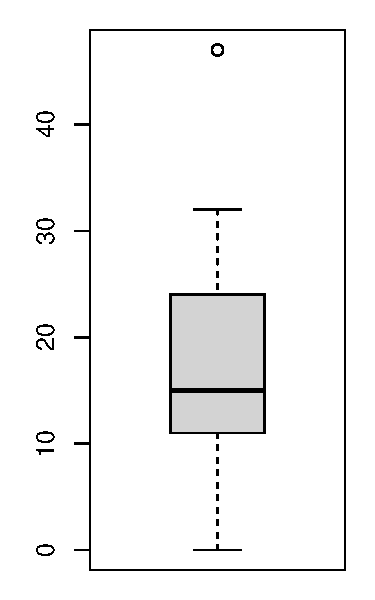
\includegraphics[scale=0.4]{figure/boxplot1.pdf}
\end{frame}

%---------------------------------------
\begin{frame}[fragile]{Histogram}
\begin{itemize}
\item A histogram is a useful way to visualize the distribution of a numerical variable.  
\vspace{10pt}
\item To construct a histogram, the range of the data is divided into bins of equal width.  Then the number of observations falling in each bin are counted.  The counts are plotted as rectangles over each bin.
\vspace{10pt}
\item Histograms are especially convenient for understanding the shape of the data distribution.
\end{itemize}
\end{frame}

%---------------------------------------
\begin{frame}[fragile]
\small
\begin{verbatim}
> sort(mtcars$mpg)
 [1] 10.4 10.4 13.3 14.3 14.7 15.0 15.2 15.2 15.5 15.8 16.4
[12] 17.3 17.8 18.1 18.7 19.2 19.2 19.7 21.0 21.0 21.4 21.4
[23] 21.5 22.8 22.8 24.4 26.0 27.3 30.4 30.4 32.4 33.9
\end{verbatim}

\begin{tabular}{l|lllll}
Bin & $(10, 15]$ & $(15, 20]$ & $(20, 25]$ & $(25, 30]$ & $(30,35]$\\
\hline
Count & 6 & 12 & 8 & 2 & 4\\
\end{tabular}

\begin{verbatim}
> hist(mtcars$mpg, main='', xlab="Miles per gallon (mpg)")
\end{verbatim}

\begin{figure}[htbp]
\centering
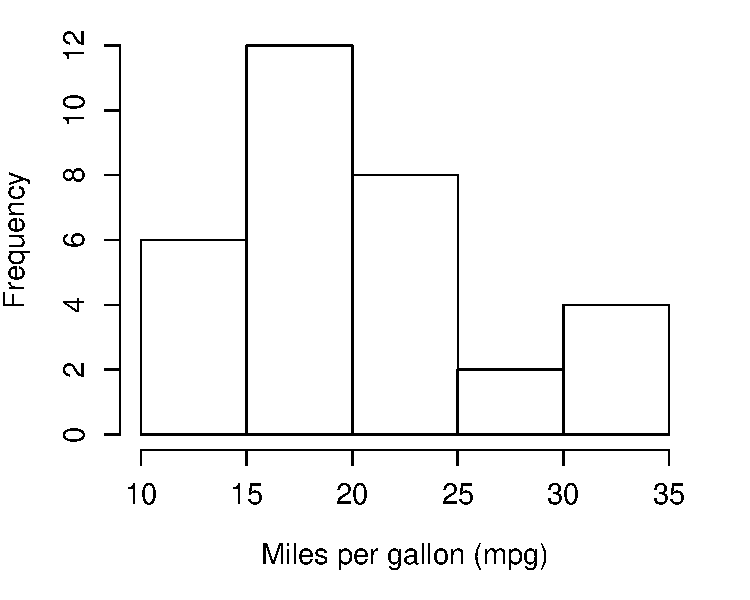
\includegraphics[width=0.5\textwidth]{figure/hist_mpg1.pdf}
\end{figure}
\end{frame}

\begin{frame}{Describing the Shape of a Distribution}
\begin{figure}[htbp]
\centering
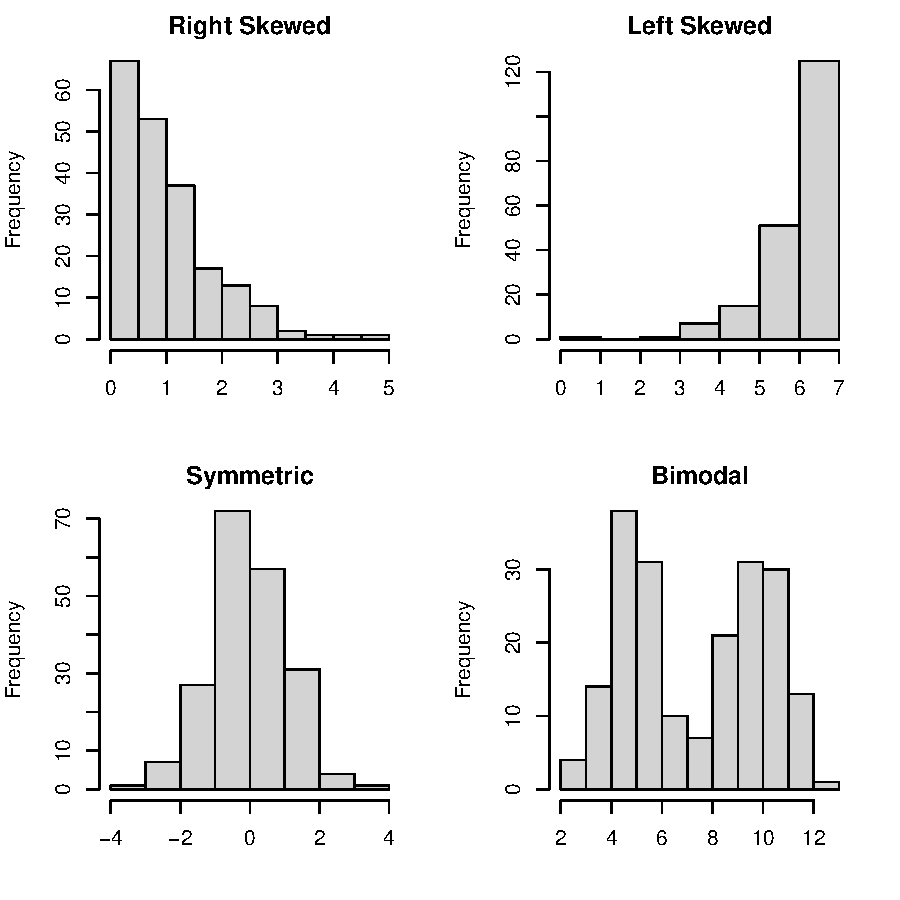
\includegraphics[scale = 0.5]{figure/shapes.pdf}
\end{figure}
\end{frame}

% \begin{frame}{Describing the Shape of a Distribution}
% \begin{itemize}
% \item When data trail off in one direction, the distribution has a \textbf{long tail}.
% \item If a distribution has a long left tail, it is called \textbf{left skewed}.  If a distribution has a long right tail, it is called \textbf{right skewed}.
% 
% \end{itemize}
% \end{frame}

\end{document}